%%%%
\newpage
\section{Poluição do Ar}

Estima-se que a poluição do ar seja responsável por 3,2 milhões de mortes 
por ano no mundo todo \citep{lim2013}, sendo as partículas, em especial, as 
de pequenas dimensões, a oferecem maiores riscos a saúde humana, pois têm 
maior facilidade de penetração no sistema respiratório.

A poluição do ar ocorre quando gases ou partículas contaminantes, 
provindas de emissões naturais ou antropogênicas, 
em suspensão na atmosfera estão em concentrações que degradam 
a qualidade do meio ambiente, afetando visibilidade, balanço energético, 
formação de nuvens ou da saúde humana, causando doenças respiratórias, 
cardiovasculares, morbidade ou até mortes. Nesta pesquisa, estuda-se somente 
a poluição causada por partículas, também chamadas de Material Particulado (MP).

%%%%
\subsection{Material Particulado}

Material Particulado (MP) é um nome dado a partículas sólidas, líquidas ou 
mistas em suspensão em um gás, no caso, a atmosfera, e têm diâmetro 
aerodinâmico equivalente compreendido entre 0,001-100 $\mu m$. A parte 
considerada inalável por seres humanos tem diâmetro menor que 10 $\mu m$
e se comporta praticamente como um gás, as partículas maiores que 10 $\mu m$ 
têm dificuldade em penetrar no sistema respiratório, porque a força de arraste 
do ar inalado através do nariz tende a não vencer a força da gravidade.

O MP pode ser classificado por tamanho, formação (primária ou secundária), 
pelas formas de remoção da atmosfera, composição química ou formato 
geométrica da partículas\citep{seinfeld2012}. A figura \ref{fig:modas_aerossol} 
é uma representação clássica das características 
do MP em função do diâmetro proposta por \citet{finlayson1999} e adaptada 
para o português por \citet{oliveira2007}, que exemplifica os processos de 
formação e remoção para cada fração. Inicialmente o MP era divido em apenas 
três modas, as partículas grossas, com  diâmetro  aerodinâmico ($\phi$) 
maior que 2,5 $\mu m$, moda de acumulação ($ 0,1\mu <\phi< 2\mu m$) e 
núcleos de Aitken ($ 0,01\mu <\phi< 0,1\mu m$). Com os avanços tecnológicos
das últimas décadas, foi possível detectar um outro grupo de partículas,
com processos de formação próprio, nucleação homogênea, e $\phi$ menor que 
0,01 $\mu m$, que devido ao tamanho, essa moda ficou conhecida como ultrafinas.

A seguir, está resumido, as características de cada moda do MP.
\begin{itemize}
\begin{spacing}{1.0}
  \item ultra-finas: formada pela nucleação homogênea de vapores de baixa 
        volatilidade;
  \item núcleos de Aitken (ou moda de nucleação): 
        gerada a partir da condensação de vapores quentes ou durante o processo 
        de transformação de gás em partícula. São removidas da atmosfera 
        por coagulação;   
  \item moda acumulação: 
        partículas na moda de acumulação são formadas a partir do crescimento 
        das partículas ultrafinas e dos núcleos núcleos de Aitken através do 
        processo de coagulação ou por condensação de vapores. São removidas da 
        atmosfera por chuva e deposição seca ou úmida.%
  \item moda grossa:
        são oriundas de processos mecânicos como fragmentação, movimentação e 
        manuseio. São removidas da atmosfera por sedimentação.
\end{spacing}
\end{itemize}

Nesta pesquisa, estudou-se o material particulado fino ($MP_{2,5}$) que 
engloba as partículas ultrafinas, núcleos de Aitken e moda de acumulação, e
o material particulado grosso ($MP_{2,5-10}$), com até 10 $\mu m$ de diâmetro, 
pois acima disso não há penetração no sistema respiratório humano. O 
$MP_{2,5-10}$ tende a sofrem maior retenção nas vias superiores, 
ficando retido na mucosa do septo do nariz, atigindo ao
máximo a nasofaringe, enquanto que $MP_{2,5}$ atinge os alvéolos pulmonares, 
bronquíolos e a corrente sanguínea, comprometendo trocas gasosas gerando
problemas cardiovasculares. O próprio corpo consegue remover partículas 
através do macrófago alveolar e do sistema linfático \citep{arbex2012}.

O MP pode ter origem primária, quando emitido diretamente na atmosfera, ou 
secundária, quando é convertido através de reações fotoquímicas, 
químicas ou físico-químicas, como por exemplo na conversão gás-partícula.
Processos naturais como ação do vento em solos e rochas, atividades vulcânicas, 
emissão biogênica (polens), poeira marinha e processos mecânicos gerais 
realizados por humanos (ex. fuligem, movimentação de veículos) emitem MP na 
fração grossa. 
Atividades antropogênicas de combustão e processos industriais, 
emitem MP na fração fina, que são compostos muitas
vezes por espécies tóxicas, como carbono elementar (ou Black Carbon), 
carbono orgânico, sulfatos ($SO_4^{2-}$) e nitratos ($NO_3^-$) (formados
secundariamente na atmosfera a partir da reação de amônia $NH_3$ com 
dióxido de enxofre $SO_2$ e óxido de nitrogênio $NO_x$, respectivamente) 
\citep{finlayson1999}. 

\newpage
\begin{figure}[H]
  \centering
  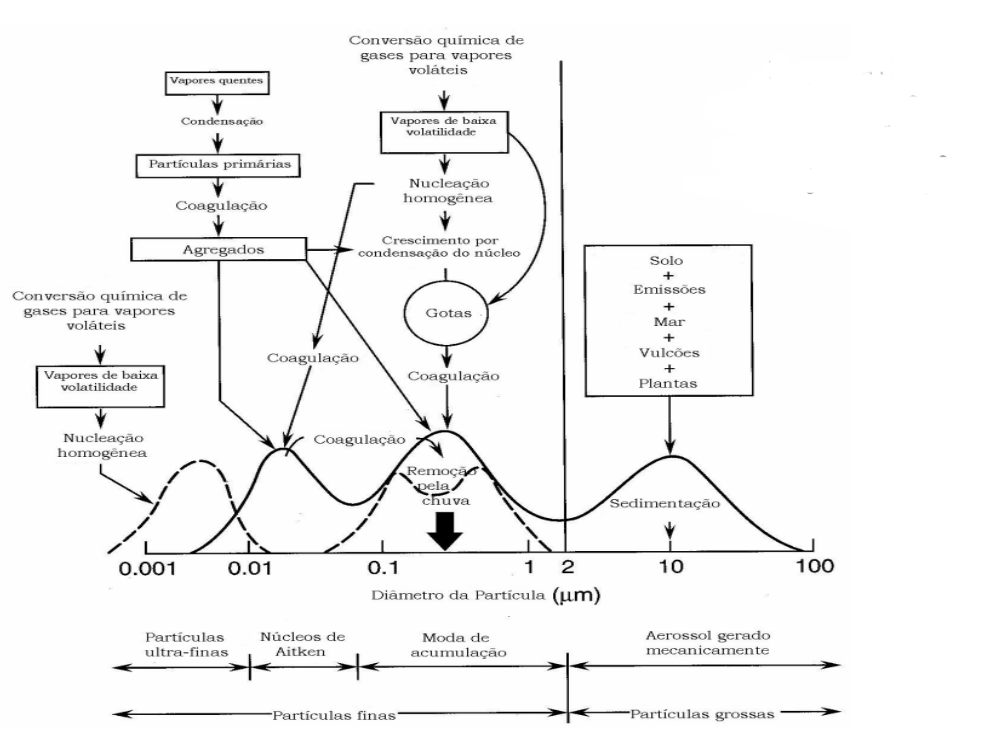
\includegraphics[width=0.8\textwidth]{../inputs/images/modas_aerossol.png}
  \caption{Esquema da distribuição de tamanho do aerossol atmosférico proposta
           por \citet{finlayson1999} e adaptada por \citet{oliveira2007} 
           \label{fig:modas_aerossol}}
\end{figure}

%%%%
\subsection{Black Carbon}

Black Carbon (BC) é um nome genérico que se da aos compostos do material 
particulado formado de carbono não orgânico e que são absorvedores de luz
visível. É formado pela combustão incompleta de combustíveis fósseis, 
biocombustível e biomassa.
Com diâmetros entre 10 e 50 nm é encontrado predominantemente na fração fina 
do material particulado e dependendo da região representa mais da metade 
da massa do $MP_{2,5}$. Por causa do seu pequeno tamanho, o BC podem atingir o
do trato respiratório inferior e segundo \citet{jacobson2014} é um dos poluentes
ambientais urbanos mais danosos a saúde humana, causando problemas respiratórios, 
cardiovasculares e morte prematura. Tanto que, desde o início de 1980, 
a Organização Mundial de Saúde (OMS) reconhecendo os efeitos do BC na saúde 
humana formulou as primeiras diretrizes para limites de exposição a BC, 
reclassificando-o de provavelmente cancerígeno para cancerígeno
\citep{scovronick2015}.

Segundo \cite{petzold2013} sua principal fonte em cidades são veículos 
automotores, especialmente os movidos a óleo combustível, que geralmente 
compoẽ uma fração menor da frota, mas que em contrapartida, tem maior 
contribuição para as concentrações totais de BC. 

Na ausência de chuva reside de 1 a 2 semanas e absorve radiação solar incidente.
Tem temperatura de vaporização perto de 4000 K e é insolúvel em água e 
solventes orgânicos comuns. Depois do dióxido de carbono é o segundo 
agente mais importante para mudança climática \citep{bond2013}.

